\documentclass{article}
\usepackage{booktabs}
\usepackage[a4paper, left=1.5in, right=1.5in, top=2in, bottom=2in]{geometry}
\usepackage{float}
\usepackage{fancyhdr}
\usepackage{amsmath}
\usepackage[nottoc]{tocbibind}
\usepackage{hyperref}
\usepackage{url}
\hypersetup{
    pdfborder = {0 0 0}
}
\fancyhf{} % Clear header/footer
\renewcommand{\headrulewidth}{0pt} % Remove header rule
\usepackage[english]{babel}

\usepackage{appendix}

\usepackage{listings}
\usepackage{xcolor}
\usepackage{color}
\usepackage{pdfpages}

\definecolor{json_string}{RGB}{160,32,240}
\definecolor{json_keyword}{RGB}{0,0,255}
\definecolor{json_number}{RGB}{0,128,0}

\lstdefinelanguage{json}{
    basicstyle=\ttfamily\footnotesize,
    numbers=left,
    numberstyle=\tiny,
    stepnumber=1,
    numbersep=5pt,
    showstringspaces=false,
    breaklines=true,
    frame=lines,
    backgroundcolor=\color{white},
    keywords=[2]{true,false,null},
    keywordstyle=[2]\color{json_keyword},
    keywords=[3]{string,number,array,object},
    keywordstyle=[3]\color{json_keyword},
    string=[b]{"},
    stringstyle=\color{json_string},
    comment=[l]{//},
    morecomment=[s]{/*}{*/},
    commentstyle=\color{gray},
    tabsize=2
}



\begin{document}

\title{RAFT consensus algorithm over a distributed Key-Value store}
\author{
Kalopisis Ioannis 7115112200011\\
Notaris  Ioannis 7115112200038}
\date{\today}


\maketitle
\thispagestyle{empty}
\newpage
\tableofcontents

\newpage

\section{Introduction}
Distributed systems have gained immense popularity in recent years due to their ability to
handle large-scale data storage and processing. Key-value stores, a fundamental building
block of many distributed systems, provide a simple and efficient way to store and retrieve
data based on unique keys. In this report, we present the design and implementation of a
key-value store that utilizes the Raft consensus algorithm for fault-tolerant replication
and consistency across a cluster of nodes.

The key-value store we have developed serves as a reliable and scalable solution for storing
and retrieving key-value pairs in a distributed environment. The system is designed to handle
high volumes of read and write requests while ensuring strong consistency guarantees.
By leveraging the Raft consensus algorithm, our system achieves fault tolerance and replication,
enabling it to operate reliably even in the face of node failures or network partitions.

The core functionality of our system revolves around the interaction between a client program,
the key-value nodes, and the Raft algorithm. Clients send messages to the key-value store,
which then forwards them to the Raft consensus algorithm. Raft ensures that the messages are
replicated across a specified number of nodes in the cluster, maintaining consistency and
fault tolerance. Once a response is obtained from the key-value nodes, it is sent back to the
client program. This process enables clients to interact seamlessly with the key-value store,
enjoying the benefits of fault tolerance, scalability, and consistency provided by the
underlying Raft algorithm.

In the following sections of this report, we will delve deeper into the design choices and
implementation details of our key-value store and the integration of the Raft consensus algorithm.
We will explore the architecture, communication protocols, and fault-tolerance mechanisms employed
in the system.  Ultimately, our goal is to present a comprehensive overview of our key-value
store and Raft implementation, showcasing the robustness and efficiency of our distributed system.

\section{RAFT consensus algorithm}
The implementation consists of two primary components: the \texttt{RaftServer} and 
the \texttt{Log} class. Together, these components implement the Raft consensus 
algorithm. The user interacts with the raft servers via an API from the cli. This report provides 
a detailed overview of 
how the Raft consensus algorithm is implemented.

\subsection{Raft Server}

The \texttt{raft\_node} class represents an individual node in the Raft consensus 
algorithm. It encapsulates the logic for managing the node's state, participating in 
leader election, replicating log entries, and handling client requests. The key features 
of the \texttt{raft\_node} class are as follows:

\begin{enumerate}
    \item Configuration: The \texttt{raft\_config} object, an instance of the IniConfig 
    class, is used to store and access configuration parameters for the Raft node. These 
    parameters include timeouts and election-related settings. Additionally, the servers 
    object, an instance of the JsonConfig class, holds the details of all servers 
    participating in the Raft cluster, such as their host addresses and ports.
    \item RPC and Communication: The Raft node utilizes the RPCClient object to 
    communicate with other nodes in the Raft cluster using remote procedure calls (RPCs). 
    This enables the node to send and receive messages for leader election, log replication, 
    and handling client requests.
    \item State and State Transitions: The \texttt{raft\_node} class maintains various state 
    variables, including the current node's role (leader, follower, or candidate), term, and 
    voted-for candidate. The node transitions between different states based on internal 
    events and external interactions with other nodes. The implementation includes methods for 
    handling state transitions, such as \texttt{start\_election}, 
    \texttt{transition\_to\_follower}, \texttt{transition\_to\_leader}, 
    \texttt{transition\_to\_candidate} etc.
    \item Leader Election: The Raft node participates in leader election by exchanging 
    messages with other nodes in the cluster. It utilizes a randomized election timeout 
    mechanism to trigger leader election if no heartbeat messages are received within the 
    timeout duration. The \texttt{raft\_node} class includes \texttt{start\_election} method 
    for initiating leader election and handling vote responses and processing vote requests 
    (\texttt{request\_vote\_rpc}).
    \item Log Replication: The \texttt{raft\_node} class implements the log replication 
    mechanism to ensure consistency across all nodes in the cluster. It includes methods for 
    appending new log entries to the log, replicating log entries to followers, and committing 
    log entries once a majority of nodes have acknowledged them. The log replication is 
    achieved through interactions with the Log class, which manages the log entries and 
    interacts with a MongoDB database for persistence.
    \item Append Entries Mechanism: The Raft consensus algorithm utilizes the append entries 
    mechanism to replicate log entries across nodes in the cluster. The main \texttt{run} 
    method is responsible for sending append entries RPCs to followers, updating their logs, 
    and ensuring consistency. The method includes parameters such as the leader's term, leader 
    ID, previous log index, previous log term, and a list of log entries to be replicated. 
    Followers validate the received entries, append them to their logs, and respond with 
    success or failure status (\texttt{append\_entries\_rpc}).
    \item Client Requests: The Raft node handles client requests by forwarding them to the 
    leader node for processing via the API.
\end{enumerate}

\subsection{Replicated Log}

The Log class is responsible for managing the log entries of the Raft node. It interacts with 
a MongoDB database to store and retrieve log entries efficiently. The key functionalities of 
the Log class are as follows:
\begin{enumerate}
    \item Initialization and Database Connection: The Log class is initialized with the 
    necessary parameters, including the database URI, database name, collection name, and 
    server ID. It establishes a connection to the MongoDB database using the provided URI and 
    initializes the collection for storing log entries.
    \item Loading and Saving Entries: The \texttt{load\_entries} method retrieves all log 
    entries from the MongoDB collection and populates the entries list of the Log instance. 
    The \texttt{save\_entry} method is used to store a new log entry in the MongoDB 
    collection.
    \item Log Entry Management: The Log class provides methods to append new log entries 
    (\texttt{append\_entry}), retrieve a specific entry by index (\texttt{get\_entry}), and 
    retrieve the last index (\texttt{get\_last\_index}) and term (\texttt{get\_last\_term}) of 
    the log. It also includes methods to mark an entry as committed (\texttt{commit\_entry}), 
    delete entries from the collection (\texttt{delete\_entry\_from\_\\collection} and 
    \texttt{delete\_entries\_after}).
    \item Committing Entries: The \texttt{commit\_entries} method is responsible for marking 
    log entries as committed within a specified range. It iterates over the entries in the 
    given range, updates their \texttt{is\_committed} flag, and updates the corresponding 
    documents in the MongoDB collection. Additionally, it invokes the 
    \texttt{append\_to\_state\_machine} method to apply the committed entries to the state 
    machine.
    \item Querying Log Entries: The \texttt{get\_all\_entries\_from\_index} method returns all 
    log entries from a specified index onwards. The \texttt{is\_empty} method checks if the 
    log is empty by examining the length of the entries list.
    \item State Machine Interaction: The \texttt{append\_to\_state\_machine} method invokes 
    the \texttt{raft\_request} RPC on the key-value store server using the 
    \texttt{kv\_store\_rpc\_client} object. This allows the log entry to be applied to the 
    state machine for further processing.
\end{enumerate}

\section{Interacting with the Raft cluster}
To interact with the Raft cluster, an API server is built on top of each Raft server to handle
user requests. These requests are made from the command line tool that we built and are essential
for the cluster to function properly. The API server provides a set of endpoints that allow users
to perform various operations such as appending log entries, retrieving log information, adding or
updating nodes, and starting or stopping the Raft cluster.

By leveraging the API server, users can seamlessly interact with the Raft cluster and manage its
configuration and state. Additionally, the API server implements basic authentication to ensure
secure access to the cluster, requiring users to provide correct credentials before performing any
operations. Overall, the API server plays a crucial role in enabling external communication with
the Raft cluster and ensuring the proper functioning of the distributed consensus algorithm. The
endpoints are described in more detail bellow.

\subsection{API Server Endpoints}

\begin{enumerate}
	\item \texttt{POST /append\_entries}: This endpoint receives the \texttt{append\_entries}
	request, which is used to replicate log entries across the Raft cluster. If the server receiving
	the request is not the leader, it forwards the request to the leader.
	\item \texttt{GET /get\_log}: This endpoint retrieves the log entries stored in the current server's log.
	\item \texttt{GET /authenticate}: This endpoint serves as a protected endpoint that requires
	authentication. It can be used to verify the correctness of the provided credentials.
	\item \texttt{POST /add\_node}: This endpoint adds a new node to the Raft cluster. It updates the
	server's configuration and saves it.
	\item \texttt{POST /update\_node}: This endpoint updates the information of an existing node in the
	Raft cluster. It modifies the server's configuration and saves it.
	\item \texttt{POST /delete\_node/{server\_id}}: This endpoint deletes a node from the Raft cluster
	based on the provided \texttt{server\_id}. If the deleted node is the current server, it stops the
	server.
	\item \texttt{GET /get\_servers}: This endpoint retrieves information about the available API servers
	and Raft servers in the cluster.
	\item \texttt{GET /get\_state}: This endpoint retrieves the current state of the Raft server, including
	the leader ID, running status, and state.
	\item \texttt{POST /start\_server}: This endpoint starts the Raft server if it is not already running.
	\item \texttt{POST /stop\_server}: This endpoint stops the Raft server if it is running
\end{enumerate}


\section{Key-Value store}
The Key-Value Store is a distributed server-based application that facilitates the storage
and retrieval of data using unique key-value pairs. It provides a simple yet powerful
abstraction for organizing and accessing data efficiently. This section provides a comprehensive
overview of the Key-Value Store application, including its purpose, architecture, functionality,
advantages, and potential use cases.

The purpose of the Key-Value Store application is to offer a scalable and efficient solution
for data storage and retrieval. By using a key-value pair approach, it enables clients to
easily store and retrieve data using unique keys.


\subsection{Architecture}
The Key-Value Store application follows a distributed architecture that ensures high availability,
fault tolerance, and scalability. Data is distributed and replicated across multiple servers,
with each server responsible for a specific portion of the key space. Clients interact with the
servers to perform operations like storing, retrieving, updating, and deleting key-value
pairs. The servers communicate with each other, through the Raft system, to maintain
data consistency and handle server failures.

\subsection{Communication}
At this section we will describe the communication between the client and the key-value server,
and the communication between the key-value server and the Raft server. Also we will describe
the message types that are exchanged between the client, key-value server, and Raft server.
In Figure \ref{fig:communication}, we can see the full path of a request from the user to
to key-value store, to raft and back to key-value store.

\begin{figure}
  \centering
  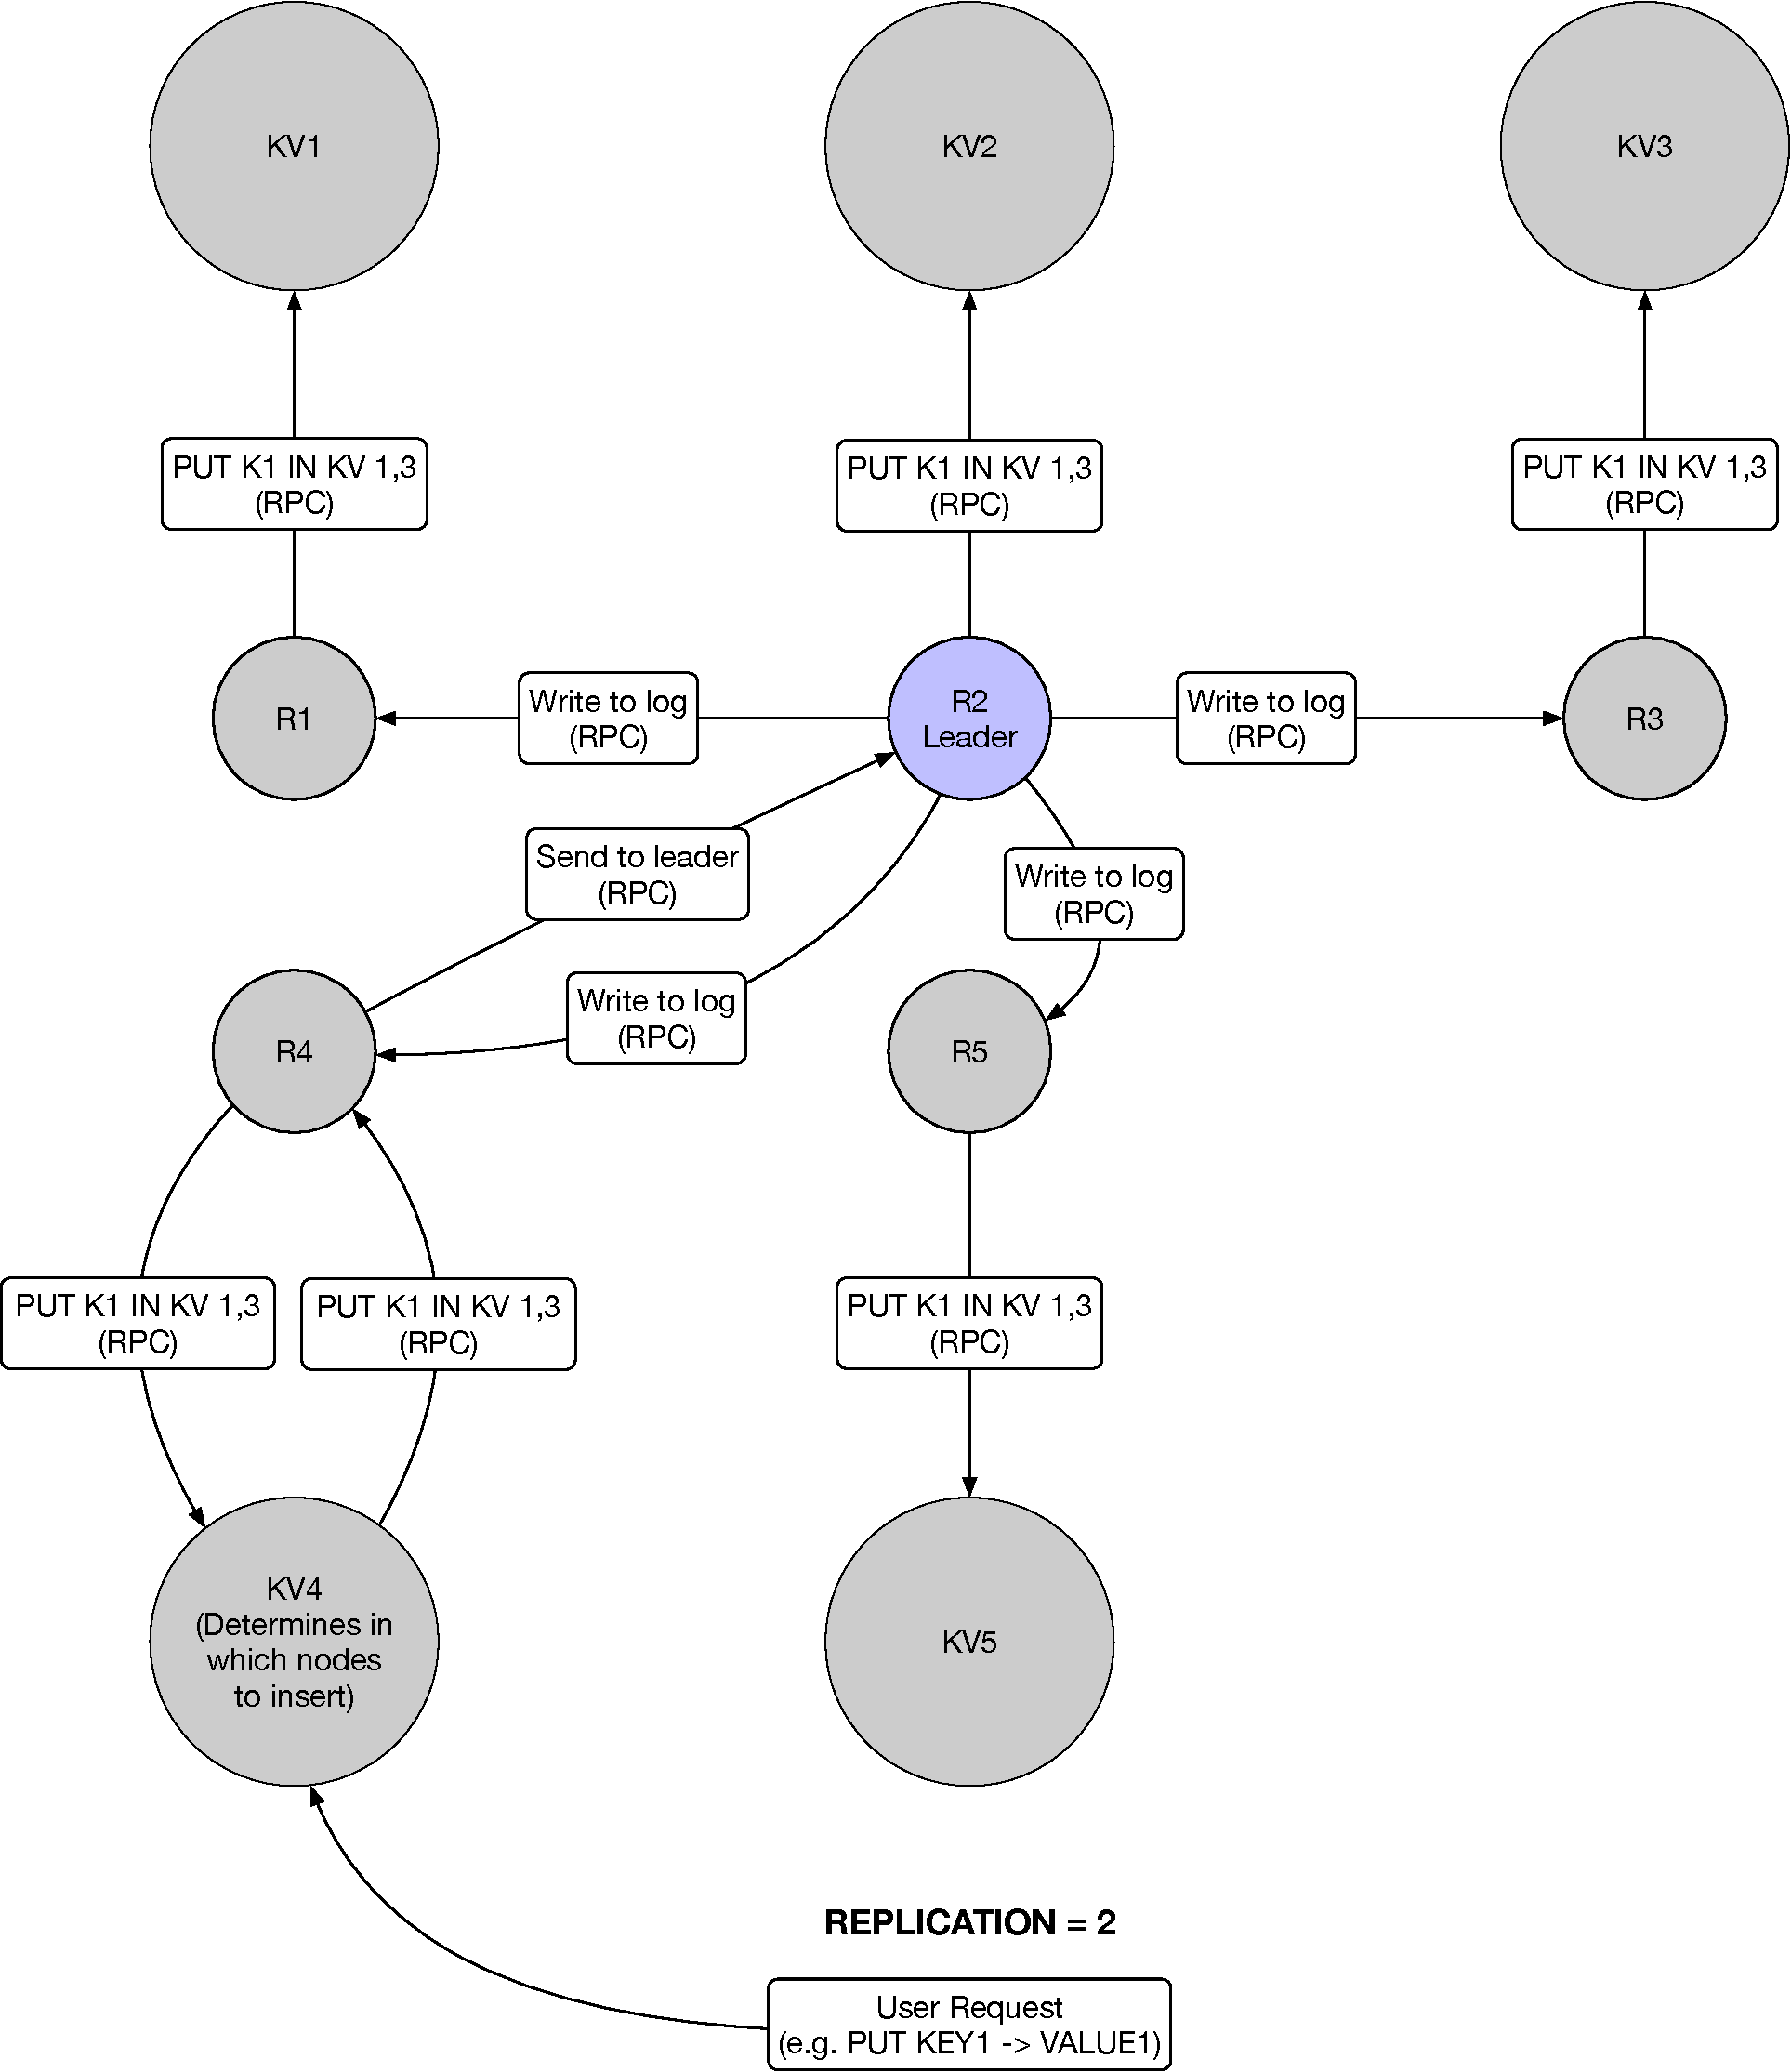
\includegraphics[width=\textwidth]{communication_diagram.pdf}
  \caption{Communication Diagram. The \texttt{PUT} request comes from the user and is sent to raft node 4.
  The raft node will forward it to leader and the leader will replicate it in all the other nodes. When a
  node gets a entry from the leader it will write it to its log and sent it to key-value store when it
  gets committed.}
  \label{fig:communication}
\end{figure}


\subsubsection{Message Types}
The client, key-value server, and Raft server exchange messages in the form of serialised JSON 
objects. Two classes were implemented to better decode, manage, and store the messages exchanged 
between the client, key-value server. These two classes are \texttt{ServerJSON} 
and \texttt{RaftJSON}. All the communication happens with the use of RPC calls. For the Key Value
Store, 4 RPC functions are registered to handle the communication from the user, other store nodes, 
and raft nodes. These functions are:

\begin{enumerate}
	\item \texttt{client\_request\_rpc} function is responsible for processing requests initiated by
	clients of the Key Value server. These requests typically involve \texttt{PUT}, \texttt{DELETE} and
	\texttt{SEARCH} operations on the key-value store, and the function ensures that the operations are
	executed correctly and provide appropriate responses to the clients. The available commands are:
		\begin{itemize}
    		\item \text{PUT}: store a key-value pair in the key-value store.
    		\item \text{DELETE}: delete a key-value pair from the key-value store.
    		\item \text{SEARCH}: retrieve a key-value pair that match the specific pattern 
    		that was given to the system
		\end{itemize}
	\item \texttt{kv\_request\_rpc} function handles requests related to the internal operations of the Key
	Value server. It may include tasks such as retrieving data from the key-value store, updating the store
	with new key-value pairs, etc.

	\item \texttt{raft\_request\_rpc} function is crucial for the integration of the Raft consensus algorithm.
	It facilitates communication between the Store and the its Raft node and handles requests related to the
	Raft protocol. This function plays a vital role in coordinating the consensus process.
		
%     RaftJSON is used for this communication. It contains an extra field, which is a list of key-value server
%     IDs, to indicate on which servers of the key-value store the data-import commands should be executed. Also
%     the commands field is, unlike ServerJSON, an array of command strings.

	\item \texttt{update\_raft\_config} function allows for dynamic updates to the Raft configuration. As the
	cluster may require changes in its membership, such as adding or removing nodes, this function ensures the
	Store reflects those changes.

\end{enumerate}

Both ServerJSON and RaftJSON messages are typically serialized into a suitable data format,
such as JSON, before transmission over the network. This allows the messages to be easily
parsed and reconstructed by the receiving party. The exchange of messages between the client,
key-value server, and Raft server enables the coordination, synchronization, and fault tolerance
mechanisms necessary for the reliable operation of the Key-Value Store application.

\begin{lstlisting}[language=json, caption={RaftJSON},label={lst:RaftJSON}]
{
    "commands": ["example command 1",
                 "example command 2",
                 "example command 3"],
    "rep_ids": [1, 5, 6]
}
\end{lstlisting}

\subsubsection{Communication Schema}
The communication schema and path between the client, key-value server, and Raft server in the
Key-Value Store application can be summarized in the following steps (see Figure~\ref{fig:communication} for
a visual representation):
\begin{itemize}
    \item \text{Client to Key-Value Server}: The client communicates with the Key-Value Server
    by sending requests over the network connection. When a client wants to store or retrieve
    a key-value pair, it sends a request to the Key-Value Server. The request is a ServerJSON
    object. The Key-Value Server receives the request and processes it by executing the
    appropriate action based on sender and the command type (PUT, DELETE, SEARCH). If the
    command type is PUT or DELETE, that is, some change should be made to the data stored on
    the servers, the Key-Value server sends the message to Raft. Once the action is completed, 
    the Key-Value Server sends a response back to the client.
    \item \text{Key-Value Server to Raft Server}: When a Key-Value Server
    receives a client request that requires updates to the key-value data, it interacts with
    the Raft Server to ensure that the updates are replicated across the cluster of Key-Value
    Servers. It sends append entries request to the Raft API Server, which includes the new entries
    to be stored.
    \item \text{Raft Server to Key-Value Server}: The Raft Server communicates with the Key-Value
    Servers to maintain coordination and provide fault tolerance. The Raft Server receives the
    payload from the append entries API call and replicates it to all Raft nodes. When a command
    gets committed each raft server will send the message to its corresponding Key-Value Server 
    to process it.
\end{itemize}

Overall, the communication between the client, key-value server, and Raft server in the Key-Value
Store application follows a distributed architecture where the client interacts directly with the
key-value server for data operations, while the key-value server interacts with the Raft server
for consistency and fault tolerance. The Raft server coordinates the replication of updates and
ensures that the key-value servers are in sync. This communication schema enables a reliable and
scalable distributed key-value storage system.


%\newpage
%\bibliographystyle{unsrt}
%\bibliography{bib.bib}

\end{document}